% !TEX program = xelatex

\documentclass[10pt,aspectratio=1610,professionalfont]{beamer}

%=========================
%        packages
%=========================
\usepackage[progressbar=frametitle]{beamerthememetropolis}
\usepackage{appendixnumberbeamer}
\usepackage{booktabs}
\usepackage{pgfplots}
\usepackage{amsmath}
\usepgfplotslibrary{dateplot}
\usepackage{xspace}
\usepackage[colorinlistoftodos]{todonotes}
\usepackage{caption}
\usepackage{subcaption}
\usepackage[many]{tcolorbox}
\usepackage{multicol}
\usepackage{multirow}
\usepackage{etoolbox}
% get environments infobox, bluehighlight, redhighlight
\newenvironment{infobox}[1]{\begin{tcolorbox}[colback=mDarkTeal!10!white,
colframe=mDarkTeal,
                     title=\textsc{#1},  
                     center, 
                     valign=top, 
                     halign=left,
                     before skip=0.8cm, 
                     after skip=1.2cm,
                     center title, 
                     outer arc=0mm,
                     boxrule=0.2pt,
                     width=\textwidth]
}{}

\newenvironment{highlightbox}[2]{
	\begin{tcolorbox}[
		colback=#1!10!white,
		colframe=#1,  
		valign=center, 
        halign=left,
        before skip=0.3cm, 
        after skip=0.5cm,
        center title, 
        arc=0mm,
		boxrule=0.2pt,
        leftrule=3mm,
        width=#2\textwidth]
       \small
}{\normalsize\end{tcolorbox}}

\newenvironment{tagbox}{\begin{tcolorbox}[colback=mLightBrown!10!white,
colframe=mLightBrown,  size=fbox]
}{\end{tcolorbox}}




%=========================
%         colors
%=========================

\definecolor{mDarkGray}{HTML}{363d41}
\definecolor{mLightGray}{HTML}{d2dadd}
\definecolor{mRed}{HTML}{CC1C14}
\definecolor{mBlue}{HTML}{203c56}
\definecolor{mGreen}{HTML}{14cc33}
\definecolor{mPurple}{HTML}{882291}
\definecolor{mTeal}{HTML}{22917d}

\setbeamercolor{background canvas}{bg=white}

%=========================
%       Title page
%=========================

\title{\textsc{Speaker Recognition in the Wild}}
\subtitle{Audio Pattern Recognition Project}
\author{Gabriele Cerizza}
\date{}
\institute{\textit{Università degli Studi di Milano}}
%\titlegraphic{\hfill\includegraphics[height=1.5cm]{logo.pdf}}

%=========================
%          Fonts
%=========================
\usepackage[no-math]{fontspec}
\setmainfont{Alegreya Sans}
 %\setmainfont[Ligatures=TeX]{Open Sans}
%\usepackage{gfsneohellenicot}
%\usepackage[default]{sourcesanspro}
\setsansfont{Alegreya Sans}
%\usefonttheme[onlymath]{serif}
\usepackage{MnSymbol}
\usepackage[MnSymbol]{mathspec}
\setmathfont(Digits,Latin)[Lowercase=Regular,Uppercase=Regular]{Alegreya Sans}
\setmathfont(Greek)[Lowercase=Regular,Uppercase=Regular,Scale=0.95]{Alegreya Sans}
\AtBeginEnvironment{align}{\large}
\AtEndEnvironment{align}{\normalsize}
\usepackage{graphicx}
\renewcommand*\partial{\textsf{\reflectbox{6}}}
\setbeamertemplate{itemize item}{\large\guillemotright\normalsize}
\setbeamertemplate{itemize subitem}{\large\guilsinglright\normalsize}





%_________________________________________
%_________________________________________

\begin{document}
\maketitle

%\begin{frame}[noframenumbering]{Outline}
% \setbeamertemplate{section in toc}[sections numbered]
%  \tableofcontents
%\end{frame}
%_______________________________________________________________________________

\section{\textsc{task overview}}

\begin{frame}{\textsc{definitions}}
    	\begin{columns}
		\begin{column}{0.5\textwidth}
			\center
			\textbf{\huge{Speaker Identification}}
			\vspace{5mm}
		   	\begin{center}
		     	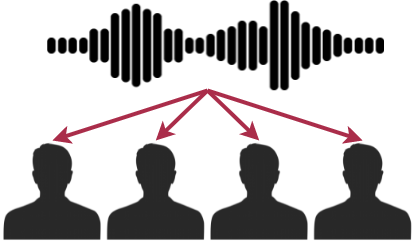
\includegraphics[width=0.8\textwidth]{img/speaker_identification.png}
		    	\end{center}
			\vspace{2mm}
			\Large{Who is the speaker?}
		\end{column}
		\begin{column}{0.5\textwidth}  %%<--- here
			\center
			\textbf{\huge{Speaker Verification}}
			\vspace{5mm}
		   	\begin{center}
		     	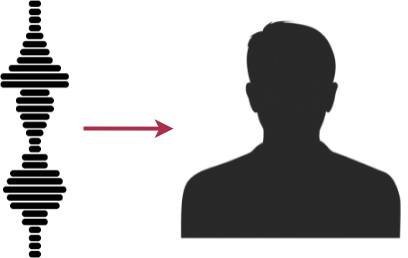
\includegraphics[width=0.8\textwidth]{img/speaker_verification.png}
		    	\end{center}
			\vspace{2mm}
			\Large{Is this speaker A?}
		\end{column}
	\end{columns}
\end{frame}

\setbeamercovered{transparent=25}
\begin{frame}{\textsc{architectures}}
	\begin{columns}
		\begin{column}{0.3\textwidth}
		   	\begin{center}
		     	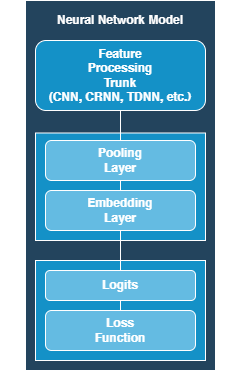
\includegraphics[width=1.1\textwidth]{img/architecture.png}
		    	\end{center}
		\end{column}
		\begin{column}{0.5\textwidth}  %%<--- here
			\begin{itemize}
		        \item \textbf{First block (``Trunk")}
		        \begin{itemize}
		            	\item Takes as input acoustic features (MFCCs or Mel spectrograms) and outputs frame-level features
		        \end{itemize}
		        \item \textbf{Second block}
			  \begin{itemize}
		             \item Pooling layer to aggregate frame-level features of varying length into fixed dimensional utterance-level features
					 \item Fully connected layer to produce embeddings
					\end{itemize}
		        \item \textbf{Third block}
		        \begin{itemize}
			\item Projection into a dimension whose size is the number of speakers 
		             \item Loss function
		        \end{itemize}
		    \end{itemize}
		\end{column}
	\end{columns}
    
\end{frame}

\setbeamercovered{invisible}
\begin{frame}{\textsc{speaker verification peculiarities}}
    \begin{itemize}
        \item \textbf{Scoring}
	  \begin{itemize}
		\item PLDA
             \item Cosine distance
        \end{itemize}
        \item \textbf{Score normalization}
	 \begin{itemize}
		\item Adaptive S-Norm
        \end{itemize}
	 \item \textbf{Metrics}
	 \begin{itemize}
		\item EER
		\item MinDCF
		\begin{equation*}
		   \hspace{-60mm}
		    C_{\text{miss}} \times P_{\text{target}} \times P_{\text{miss}}(\theta) +
		    C_{\text{fa}} \times (1 - P_{\text{target}}) \times P_{\text{fa}}(\theta) 
		\end{equation*}
        \end{itemize}
    \end{itemize}
\end{frame}

\begin{frame}{\textsc{pooling layers}}
	\begin{columns}
		\begin{column}{0.4\textwidth}
		\begin{itemize}
	        \item \textbf{Temporal Average Pooling (TAP)}
		  \item \textbf{Self-Attentive Pooling (SAP)}
	%	  \vspace{2mm}
	%	  \begin{equation*}
	%  	    \hspace{-80mm}
	%	    h_t = \text{tanh}(Wx_t + b)
	%	\end{equation*}
	%	\begin{equation*}
	%	   \hspace{-80mm}
	%	    w_t = \frac{\text{exp}(h_t^T\mu)}{\sum_{t=1}^T\text{exp}(h_t^T\mu)}
	%	\end{equation*}
	%	\begin{equation*}
	%	    \hspace{-80mm}
	%	    e = \sum_{t=1}^Tw_tx_t
	%	\end{equation*}
		\item \textbf{Other Pooling Layers}
	        \begin{itemize}
	            \item Self Multi-Head Attention Pooling
	            \item Attentive Statistics Pooling (ASP) 
	        \end{itemize}
	    \end{itemize}
		\end{column}
		\begin{column}{0.3\textwidth} 
		\begin{center}
		     	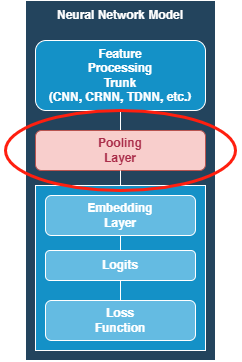
\includegraphics[width=1.1\textwidth]{img/pooling_layer.png}
		    	\end{center}
		\end{column}
	\end{columns}
    
\end{frame}

\begin{frame}{\textsc{loss functions}}
    \begin{columns}
		\begin{column}{0.4\textwidth}
		\begin{itemize}
	        \item \textbf{Softmax}
		  \begin{itemize}
	            \item  Does not enforce intra-class compactness and inter-class separation
	        \end{itemize}
		  \item \textbf{Angular Additive Margin Softmax (AAM Softmax)}
		  \begin{itemize}
		      \item Improves compactness and separation
	            \item  Difficult to train with and sensitive to parameters
	        \end{itemize}
		  \item \textbf{Sub-center Angular Additive Margin Softmax (SC AAM Softmax)}
		   \begin{itemize}
	            \item  More robust against noisy data
	        \end{itemize}
	    \end{itemize}
		\end{column}
		\begin{column}{0.6\textwidth} 
		\begin{center}
		     	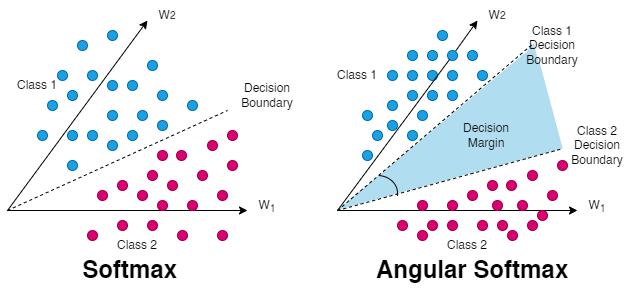
\includegraphics[width=1.0\textwidth]{img/softmax.png}
		    	\end{center}
		\end{column}
	\end{columns}
    
\end{frame}

\section{\textsc{experiment}}

\begin{frame}{\textsc{dataset}}
	 \begin{columns}
		\begin{column}{0.5\textwidth}
		 \begin{itemize}
	        \item \textbf{VoxCeleb1 Dataset}
	        \begin{itemize}
	            \item Collected “in the wild" from Youtube
	            \item Background noise, music, overlapping speech and varying room acoustics
	            \item Heterogeneous age, gender and nationality 
	        \end{itemize} 
	        \item \textbf{We used a subset due to hardware constraints}
	        \begin{itemize}
	            \item 100 speakers, retaining gender ratio
		      \item Official training, validation and test splits
		      \item For verification,	 10 speakers not present in the training set 
	        \end{itemize}
	    \end{itemize}
		\end{column}
		\begin{column}{0.5\textwidth} 
		\begin{center}
		     	\begin{table}[htbp]
			    \begin{center}
				 \resizebox{0.9\textwidth}{!}{
			        \begin{tabular}{|c|c|c|c|c|}
			        \cline{3-5}
			        \multicolumn{2}{c|}{\textbf{}} & \textbf{Full Dataset} & \textbf{Identif. Set} & \textbf{Verif. Set}\\
			        \hline
			        \multicolumn{2}{|c|}{\textbf{Speakers No.}} & 1,251 & 100 & 10\\
			        \hline
			        \multicolumn{2}{|c|}{\textbf{Samples No.}} & 152,123 & 12,123 & 1,896 \\
			        \hline
			        \multirow{2}{*}{\textbf{Gender}} & \textit{Male} & 0.55 & 0.51 & 0.50 \\
			        & \textit{Female} & 0.55 & 0.52 & 0.50 \\
			        \hline
			        \multirow{4}{*}{\textbf{Nationality}$^{\mathrm{a}}$} & \textit{USA} & 0.65 & 0.52 & 0.41 \\
			        & \textit{UK} & 0.21 & 0.12 & 0.32 \\
			        & \textit{Italy} & 0.01 & 0.05 & 0.07 \\
			        & \textit{Russia} & 0.07 & 0.02 & 0.02 \\
			        \hline
			        \multirow{2}{*}{\textbf{Seconds}} & \textit{Mean} & 8.12 & 7.59 & 5.67 \\
			        & \textit{Std} & 2.55 & 3.55 & 4.55 \\
			        \hline
			        \multicolumn{4}{l}{$^{\mathrm{a}}$Only the four most frequent nationalities are listed.}
			        \end{tabular}
				}
			        \label{tab:dataset}
			    \end{center}
			\end{table}
		\end{center}
		\end{column}
	\end{columns}
   
\end{frame}

\begin{frame}{\textsc{features and data augmentation}}
    \begin{itemize}
        \item \textbf{Features}
        \begin{itemize}
            \item 80-dimensional log Mel spectrograms
            \item Window length of 25 ms, frame-shift of 10 ms
            \item Cepstral mean normalization  
        \end{itemize} 
        \item \textbf{Offline data augmentation}
        \begin{itemize}
            \item Speed perturbation
		\item Background noise
		\item Babble
		\item Reverberation 
        \end{itemize}
        \item \textbf{Online data augmentation}
        \begin{itemize}
            \item SpecAugment: time and frequency masking
        \end{itemize} 
    \end{itemize}
\end{frame}

\begin{frame}{\textsc{models}}
     \begin{columns}
		\begin{column}{0.33\textwidth}
			\begin{center}
				\textbf{\large{ResNet34-SE}}
		     		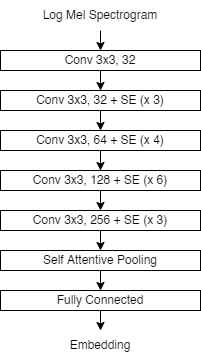
\includegraphics[width=0.8\textwidth]{img/resnet34se.png}
		    	\end{center}
		\end{column}
		\begin{column}{0.33\textwidth}
			\begin{center}
				\hspace{-7.5mm}\textbf{\large{LAS-MHA}}
		     		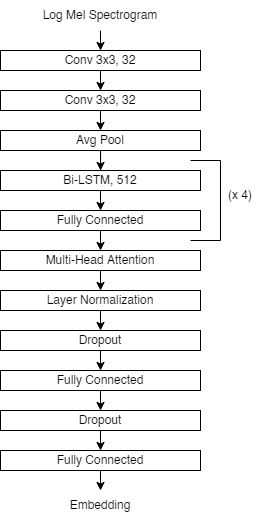
\includegraphics[width=0.8\textwidth]{img/las_mha.png}
		    	\end{center}
		\end{column}
		\begin{column}{0.33\textwidth}
			\begin{center}
				\textbf{\large{EfficientNetV2}}
		     		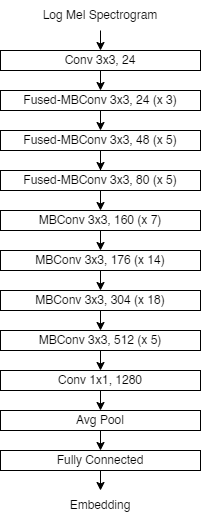
\includegraphics[width=0.6\textwidth]{img/efficientnetv2.png}
		    	\end{center}
		\end{column}
	\end{columns}
\end{frame}

\begin{frame}{\textsc{large margin fine-tuning}}
\center
    \begin{itemize}
        \item \textbf{Large margin fine-tuning} 
        \begin{itemize}
	     \item Training in two steps
            \item Random crops: from 2 to 4 seconds
		\item SC AAM Softmax: margin from 0.1 to 0.3, scale from 15 to 30
		\item SpecAugment only in the first step
        \end{itemize} 
        \item \textbf{Evaluation}
	 \begin{itemize}
            \item Full-length utterances for verification
		\item Random 4 seconds crops for identification
        \end{itemize}
    \end{itemize}
\end{frame}

\begin{frame}{\textsc{results}}
    \begin{table}[htbp]
    \begin{center}
	 \resizebox{0.7\textwidth}{!}{
        \begin{tabular}{|c|c|c|c|c|c|c|c|}
        \hline
        \textbf{Model} & \textbf{Year} & \textbf{Training Set} &  \textbf{Top1 Acc.} & \textbf{Top5 Acc.} & \textbf{F1 Score} & \textbf{EER(\%)} & \textbf{MinDCF}$^{\mathrm{a}}$\\
        \hline
        Nagrani et al. & 2017 & VoxCeleb1 & 80.5 & 92.1 & - & - & - \\
        Nagrani et al. & 2017 & VoxCeleb1 & - & - & - & 7.8 & 0.71 (0.01) \\
        Cai et al. & 2018 & VoxCeleb1 & 89.9 & 95.7 & - & - & - \\
        Cai et al. & 2018 & VoxCeleb1 & - & - & - & 5.27 & 0.439 \\
        Cai et al. & 2018 & VoxCeleb1 & - & - & - & 4.46 & 0.577 \\
        Chung et al. & 2018 & VoxCeleb1 & - & - & - & 7.8 & 0.71 (0.01) \\
        Okabe et al. & 2018 & VoxCeleb1 & - & - & - & 3.85 & 0.406 (0.01) \\
        Hajibabaei, Dai & 2018 & VoxCeleb1 & 94.6 & 98.1 & - & 4.69 & 0.453 (0.01) \\
        Hajibabaei, Dai & 2018 & VoxCeleb1 & 92.8 & 97.5 & - & 4.30 & 0.413 (0.01) \\
        India et al. & 2019 & VoxCeleb1 & - & - & - & 4.0 & 0.0045 (0.01) \\
        Chung et al. & 2019 & VoxCeleb1 & 89.00 & 96.15 & - & 5.37 & - \\
        Chung et al. & 2019 & VoxCeleb1 & 89.00 & 95.94 & - & 5.26 & - \\
        Hajavi, Etemad & 2021 & VoxCeleb1 & - & - & - & 3.14 & - \\
        Kwon et al. & 2021 & VoxCeleb2 & - & - & - & 0.73 & 0.056 (0.05)\\
        Kwon et al. & 2021 & VoxCeleb2 & - & - & - & 0.74 & 0.061 (0.05)\\
        Thienpondt et al. & 2021 & VoxCeleb2 & - & - & - & 0.64 & 0.0700 (0.01) \\
        Thienpondt et al. & 2021 & VoxCeleb2 & - & - & - & 0.56 & 0.0743 (0.01) \\
        Zhao et al. & 2021 & VoxCeleb2 & - & - & - & 0.5249 & 0.0498 (0.01) \\
        Zhao et al. & 2021 & VoxCeleb2 & - & - & - & 0.5594 & 0.0480 (0.01) \\
        \hline
        \multicolumn{8}{l}{$^{\mathrm{a}}$If provided, we noted the $P_{\text{target}}$ value within parentheses.} \\
        \end{tabular}
        }
    \end{center}
\end{table}
    
\end{frame}




\begin{frame}[standout]
    Thank You
\end{frame}


\end{document}
